\documentclass{anstrans}
%%%%%%%%%%%%%%%%%%%%%%%%%%%%%%%%%%%
\title{Unstructured CMFD Capability in MPACT}
\author{Brendan Kochunas,$^{*}$ Ben C. Yee,$^{*}$ and Michael Jarrett$^{*}$}

\institute{
$^{*}$University of Michigan, 2355 Bonisteel Blvd, Ann Arbor, MI 48109,
bkochuna@umich.edu, bcyee@umich.edu, jarremic@umich.edu
}

%%%% packages and definitions (optional)
\usepackage{graphicx} % allows inclusion of graphics
\usepackage{booktabs} % nice rules (thick lines) for tables
\usepackage{microtype} % improves typography for PDF

\usepackage{tikz}
\usetikzlibrary{arrows.meta}
\tikzset{edge/.style = {->,-{Latex[width=2mm]}}}
\usetikzlibrary{calc} %coordinate calculations

\setcounter{secnumdepth}{3}

\renewcommand{\bar}[1]{\overline{#1}} %pretty over-bars
\renewcommand{\vec}[1]{\bm{#1}}       %vector is bold italic
\newcommand{\vd}{\bm{\cdot}}          %slightly bold vector dot
\newcommand{\grad}{\vec{\nabla}}      %gradient
\newcommand{\vr}{\vec{r}}             %shortcut for vector r
\newcommand{\vOmega}{\vec{\Omega}}    %shortcut for vector Omega
\newcommand{\vJ}{\vec{J}}             %shortcut for vector J
\newcommand{\half}{\frac{1}{2}}

\renewcommand{\eqref}[1]{Eq.~(\ref{#1})}
\newcommand{\figref}[1]{Fig.~\ref{#1}}

\begin{document}
%%%%%%%%%%%%%%%%%%%%%%%%%%%%%%%%%%%%%%%%%%%%%%%%%%%%%%%%%%%%%%%%%%%%%%%%%%%%%%%%
\section{Introduction}
Recently, the modeling capability in MPACT \cite{MPACT2016} was extended to boiling water reactors (BWRs) \cite{Kochunas2017}. One aspect to modeling BWR assemblies is to account for the evolution of the fuel assembly designs. Because of operating experience and improvements in simulation capabilities, BWR fuel design has been continually evolving. Initial fuel designs consisted of 7x7 lattices, and these have evolved through 8x8, 9x9, 10x10, and most recently to 11x11 designs.

Most light water reactor neutronics analysis tools use coarse mesh finite difference (CMFD) acceleration for efficient convergence. In these CMFD implementations the coarse mesh is derived from the pin cells. Generally, using the pin cells within a lattice as the basis for the coarse mesh is a good choice as it is both natural and is likely to result in neutron net currents at the coarse mesh interfaces that are small.

As a result of this evolution in BWR fuel designs, it necessarily creates real world geometries that have mixed lattices (e.g. 8x8 next to 9x9). Given this situation and the conventional implementation of CMFD, this leads to a situation where there is now an unstructured or semi-structured interface between CMFD nodes. For traditional whole core reactor analysis methods employing the two-step procedure this is not a concern since the lattice calculation is performed in isolation. However, for high fidelity reactor simulators such as MPACT the unstructured interfaces must be treated. Such methods have been previously developed in DeCART \cite{Thomas2006,CHO2008}, NEWT \cite{Kim2011}, and likely CASMO-4\cite{Smith2002}; although the details of the latter are not explicitly described in open literature. The former provide the basis for the approach implemented in MPACT.

The remainder of this manuscript provides an overview of the theory and numerical results that verify the implementation and demonstrate the capability for a real world problem.

%%%%%%%%%%%%%%%%%%%%%%%%%%%%%%%%%%%%%%%%%%%%%%%%%%%%%%%%%%%%%%%%%%%%%%%%%%%%%%%%
\section{Theory}
The equations for unstructured CMFD are not substantially different from the structured CMFD equations. The only difference is that the calculation of surface quantities such as net and partial current must correctly account for multiple neighbors and fractional overlap between neighboring cells. We start by briefly deriving the CMFD equations for the typical structured mesh scenario and then show how these may be extended for general unstructured mesh applications. Fundamentally, the CMFD equations represent a balance equation, where the neutron balance within each node is preserved. This principle guides modification of CMFD for the case of an unstructured grid.

\subsection{Structured Coarse Mesh Finite Difference} \label{subsec:sCMFD}
The CMFD equations are derived similarly to finite volume methods. Starting from the multigroup 2D continuous transport equation with isotropic scattering:

\begin{multline} \label{eq:bte}
  \vOmega \vd \grad \psi_g(\vr,\vOmega) + \Sigma_{t,g}(\vr) \psi_g(\vr,\vOmega)
\\ =
  \frac{1}{4\pi} \bigg(\sum_{g'} \Sigma_{s,g' \rightarrow g}(\vr) \phi_{g'}(\vr)
\\  + \frac{\chi_g(\vr)}{k_{\text{eff}}} \sum_{g'} \nu\Sigma_{f,g'}(\vr)\phi_{g'}(\vr) \bigg) .
\end{multline}

First \eqref{eq:bte} is integrated over $(\vOmega)$. This results in the neutron balance equation \eqref{eq:balance}. In the following equation we simplify the right hand side to $Q_g(\vr)$.

\begin{equation} \label{eq:balance}
    \grad \vd \vJ_g(\vr) + \Sigma_{t,g}(\vr) \phi_g(\vr) = Q_g(\vr) .
\end{equation}

To obtain the low order CMFD operator, the Fick's law expression for the current is added and subtracted to the left hand side of \eqref{eq:balance}, resulting in the low order non-linear diffusion acceleration equations.

\begin{subequations} \label{eq:nda}
    \begin{multline}
        -\grad \vd D_g(\vr)  \grad\phi_g(\vr)
    + \bigg(\hat{D}_g(\vr) + \Sigma_{t,g}(\vr)\bigg) \phi_g(\vr) = Q_g(\vr) ,
    \end{multline}
    \begin{equation} \label{eq:dhatdef}
        \hat{D}_{g}(\vr) = \grad \vd \Bigg[ \vJ_g(\vr) + D_g(\vr)  \grad\phi_g(\vr)
        \Bigg] \Bigg/ \phi_g(\vr) ,
    \end{equation}
\end{subequations}

\noindent where $D_g(\vr)$ is simply $\big[3\Sigma_{t,g}(\vr)\big]^{-1}$. Next we introduce the coarse mesh in \figref{fig:mesh}. For simplicity and clarity the mesh in this figure are illustrated in 2D. Using the convention of the structured mesh on the left we discretize \eqref{eq:nda} with a finite volume approach. 

\begin{figure}[!h]
    \centering
    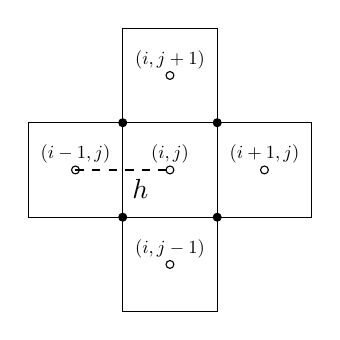
\begin{tikzpicture}
        \newcommand{\p}{1.2}
        \newcommand{\tscale}{0.67}
        \draw ( 0, 0) -- (\p, 0) -- (\p,\p) -- ( 0,\p) -- ( 0, 0); %center
        \draw ( 0,\p) -- (\p,\p) -- (\p,2*\p) -- ( 0,2*\p) -- ( 0,\p); %north
        \draw ( 0,-\p) -- (\p,-\p) -- (\p,0) -- (0,0) -- (0,-\p); %south
        \draw (-\p, 0) -- ( 0, 0) -- ( 0,\p) -- (-\p,\p) -- (-\p, 0); %left
        \draw (\p, 0) -- (2*\p, 0) -- (2*\p,\p) -- (\p,\p) -- (\p, 0); %left
        
        \draw (0.5*\p,0.5*\p) circle (0.05);
        \draw (1.5*\p,0.5*\p) circle (0.05);
        \draw (0.5*\p,1.5*\p) circle (0.05);
        \draw (-0.5*\p,0.5*\p) circle (0.05);
        \draw (0.5*\p,-0.5*\p) circle (0.05);
        
        \draw[dashed] (-0.5*\p,0.5*\p) -- (0.5*\p,0.5*\p);
        \node[anchor=north west] (p) at (0,0.5*\p){$h$};
        
        \filldraw[fill=black] (0,0) circle (0.05);
        \filldraw[fill=black] (0,\p) circle (0.05);
        \filldraw[fill=black] (\p,0) circle (0.05);
        \filldraw[fill=black] (\p,\p) circle (0.05);

        \begin{scope}[scale=\tscale, transform shape]
            \node[anchor=south]  (ij) at (0.5*\p/\tscale,0.5*\p/\tscale){$(i,j)$};
            \node[anchor=south] (ij+1) at (0.5*\p/\tscale,1.5*\p/\tscale){$(i,j+1)$};
            \node[anchor=south] (ij-1) at (0.5*\p/\tscale,-0.5*\p/\tscale){$(i,j-1)$};
            \node[anchor=south] (i+1j) at (1.5*\p/\tscale,0.5*\p/\tscale){$(i+1,j)$};
            \node[anchor=south] (i-1j) at (-0.5*\p/\tscale,0.5*\p/\tscale){$(i-1,j)$};
        \end{scope}
    \end{tikzpicture}
    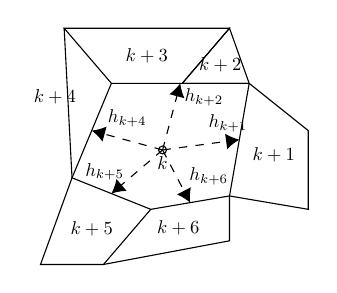
\begin{tikzpicture}
        \newcommand{\tscale}{0.67}
    
        % Vertices
        \newcommand{\pa}{(0,0)}
        \newcommand{\pb}{(1,0.17)}
        \newcommand{\pc}{(1.25,1.6)}
        \newcommand{\pd}{(-0.5,1.6)}
        \newcommand{\pe}{(-1,0.4)}
        \newcommand{\pf}{(0.4,1.6)}
        \newcommand{\pg}{(1,2.3)}
        \newcommand{\ph}{(-1.1,2.3)}
        
        \newcommand{\pj}{(-1.4,-0.7)}
        \newcommand{\pk}{(-0.6,-0.7)}
        \newcommand{\pl}{(1,-0.4)}
        
        \newcommand{\pn}{(2,1)}
        \newcommand{\po}{(2,0)}
        
        % Centroids
        \newcommand{\ca}{(0.15/\tscale,0.754/\tscale)}
        \newcommand{\cb}{(1.5625/\tscale,0.6925/\tscale)}
        \newcommand{\cc}{(0.8833/\tscale,1.833/\tscale)}
        \newcommand{\cd}{(-0.05/\tscale,1.95/\tscale)}
        \newcommand{\ce}{(-0.866/\tscale,1.433/\tscale)}
        \newcommand{\cf}{(-0.75/\tscale,-0.25/\tscale)}
        \newcommand{\cg}{(0.35/\tscale,-0.2325/\tscale)}
        
        \draw \pa -- \pb -- \pc -- \pd -- \pe -- \pa;
        \draw \pf -- \pg -- \pc -- \pf;
        \draw \pd -- \ph -- \pg -- \pf;
        \draw \ph -- \pe;
        \draw \pe -- \pj -- \pk -- \pa;
        \draw \pk -- \pl -- \pb;
        \draw \pb -- \po -- \pn -- \pc; 
        
        \begin{scope}[scale=\tscale, transform shape]
            \node[anchor=north]   (k) at \ca{$k$};
            \node[anchor=center] (k+1) at \cb{$k+1$};
            \node[anchor=center] (k+2) at \cc{$k+2$};
            \node[anchor=center] (k+3) at \cd{$k+3$};
            \node[anchor=east] (k+4) at \ce{$k+4$};
            \node[anchor=center] (k+5) at \cf{$k+5$};
            \node[anchor=center] (k+6) at \cg{$k+6$};
            \draw \ca circle (0.075);
            %\filldraw[fill=black] \ca circle (0.075);
            \draw[edge,dashed] \ca -- node[label=0:$h_{k+6}$] {} (0.5/\tscale,0.085/\tscale);
            \draw[edge,dashed] \ca -- node[label=80:$h_{k+1}$] {} (1.125/\tscale,0.885/\tscale);
            \draw[edge,dashed] \ca -- node[label=30:$h_{k+2}$] {} (0.375/\tscale,1.6/\tscale);
            \draw[edge,dashed] \ca -- node[label=90:$h_{k+4}$] {} (-0.75/\tscale,1/\tscale);
            \draw[edge,dashed] \ca -- node[label=180:$h_{k+5}$] {} (-0.5/\tscale,0.2/\tscale);
        \end{scope}
    \end{tikzpicture}
    \caption{Structured Mesh (left), Unstructured Mesh (right)}
    \label{fig:mesh}
\end{figure}

In this procedure each term in \eqref{eq:nda} is integrated over the volume %$\overline{abcd}$
for cell $i,j$. This leads to the following cell-averaged definitions of the scalar flux and cross sections this gives:
\begin{subequations} \label{eq:homcoef}
    \begin{equation}
        \bar\phi_{g,i,j} = \int_V \phi_g(\vr) d\vr ,
    \end{equation}
    \begin{equation}
        \bar\Sigma_{x,g,i,j} = \frac{1}{\bar\phi_{g,i,j}} \int_V \Sigma_{x,g}(\vr) \phi_g(\vr) d\vr ,
    \end{equation}
    \begin{equation}
        \bar\chi_{g,i,j} = \int_V \chi_g(\vr)\nu\Sigma_{f,g}(\vr) \phi_g(\vr) d\vr \Bigg/
           \int_V \nu\Sigma_{f,g}(\vr) \phi_g(\vr) d\vr ,
    \end{equation}
\end{subequations}
\noindent here $\Sigma_{x,g}$ is any one of $\Sigma_{t,g}$, $\nu\Sigma_{f,g}$, or $\Sigma_{s,g' \rightarrow g}$.

For the leakage terms, the divergence theorem results in surface quantities. Since it is assumed that the cross sections are only constant within a volume, the diffusion coefficient at the surface is not straightforwardly defined. The traditional way to obtain the diffusion coefficient at a surface, $\tilde D$, is by current continuity and a first order finite difference approximation applied to Fick's Law. This yields the following harmonic average:
\begin{equation} \label{eq:dtil}
    \tilde D_{g,i\pm\half,j} = \frac{2\bar D_{g,i,j} \bar D_{g,i\pm1,j}}
        {h \Big(\bar D_{g,i,j} + \bar D_{g,i\pm1,j}\Big)} .
\end{equation}
\noindent \eqref{eq:dtil} is for the surfaces perpendicular to the $x$-axis (e.g. the $x$ surfaces). The equations for the $y$ surfaces simply move the $\pm$ onto the $j$ subscripts. The discretized $\hat D_{g}$ is obtained similarly from \eqref{eq:dhatdef}, but utilizes the ad-hoc relationship $\bar\phi_{g,i\pm\half,j} = \bar\phi_{g,i\pm1,j} + \bar\phi_{g,i,j}$ to yield:
\begin{equation} \label{eq:dhat}
    \hat D_{g,i\pm\half,j} = \frac{J_{g,i\pm\half,j} 
         \pm \tilde D_{g,i\pm\half,j}\Big(\bar\phi_{g,i\pm1,j}-\bar\phi_{g,i,j}\Big)}
        {\Big(\bar\phi_{g,i\pm1,j}+\bar\phi_{g,i,j}\Big)} .
\end{equation}
\noindent In \eqref{eq:dhat} the $J$ term is computed from the transport solution, thus enforcing equivalence between the currents on the low-order operator and high-order transport equation.
The resulting discretized CMFD equation is then written as:
\begin{multline} \label{eq:sCMFD}
    - \sum_{s=N,S,E,W} A_{i,j}^{s}\bigg(\tilde D_{g,i,j}^s + \hat D_{g,i,j}^s\bigg) \bar{\phi}_{g,i,j}^s \\
    + \sum_{s=N,S,E,W} A_{i,j}^{s}\bigg(\tilde D_{g,i,j}^s - \hat D_{g,i,j}^s\bigg) \bar\phi_{g,i,j} \\
    + V_{i,j}\bar\Sigma_{t,g,i,j}\bar\phi_{g,i,j} = V_{i,j} \bar Q_{g,i,j} ,
\end{multline}
\noindent here we have introduced the superscript $s$ to indicate the $North$, $South$, $East$, and $West$ neighbors and replace $\Big(i\pm\half,j\Big)$ and $\Big(i,j\pm\half\Big)$ for the surface quantities and $\Big(i\pm1,j\Big)$ and $\Big(i,j\pm1\Big)$ for the cell centered quantities.

\subsection{Unstructured CMFD}
In an unstructured CMFD method, the only step that changes from the derivation in \S\ref{subsec:sCMFD} is the final step where the mesh is defined and \eqref{eq:nda} is discretized. A more general unstructured mesh is illustrated by \figref{fig:mesh} on the right.

There are two specific deviations from the structured mesh case. The first feature is the generalization of cells from squares to arbitrary polygons. Previous works \cite{CHO2008,Kim2011} describe "unstructured" treatments for the discretized CMFD problem. However, in these methods, a rigorous discretization of the unstructured diffusion equation is not performed. Therefore, some issues may be encountered in these methods that are discussed in the remainder of this section. The second feature of this unstructured mesh is the inclusion of multiple neighbors on a single face; the methodology for this is also previously described in \cite{Thomas2006}.

\subsubsection{Dealing with arbitrary polygons}
In \ref{subsec:sCMFD} we note that traditional CMFD simply declares the relationship of the surface flux to the cell centered fluxes in a way that is not wholly consistent with the rest of the procedure used to discretize \eqref{eq:nda}. The result of such an approach is that the error from the inconsistent discretization gets captured by $\hat D_g$. The CMFD and non-linear diffusion acceleration methods rely heavily on the condition that $\hat D_g$ be small. If inconsistent discretizations are used, this is less likely to be the case. This observation that consistent discretizations are necessary for effective diffusion acceleration was hard learned in the development of robust diffusion synthetic acceleration methods some years ago. However, it would be remiss not to acknowledge that in spite of an ad-hoc discretization, CMFD has been used quite successfully since its inception.

Yet we note, with some emphasis, that in the original CMFD reference \cite{Smith2002}, some special treatments or "fix-ups" are utilized. Smith and Rhodes mention that a "limiter" is placed on $\hat D_g$ to ensure the system of equations is diagonally dominant. Consequently, this likely reduces the effectiveness of CMFD in practice. By using a rigorous and consistent discretization of \eqref{eq:nda} we suggest that such fix-ups are likely not needed, and the method should perform more efficiently and robustly.

Starting from the approaches of \cite{CHO2008} and \cite{Kim2011} for unstructured CMFD, the usual definition of the current, which rearranges \eqref{eq:dhat}, is given as:
\begin{multline} \label{eq:CMFDJ}
    J_{g,i\pm\half,j} = \pm \tilde D_{g,i\pm\half,j}\Big(\bar\phi_{g,i\pm1,j}-\bar\phi_{g,i,j}\Big) \\
       + \hat D_{g,i\pm\half,j} \Big(\bar\phi_{g,i\pm1,j}+\bar\phi_{g,i,j}\Big) .
\end{multline}
In this way, the derivations in \cite{CHO2008} and \cite{Kim2011}, are similar to \cite{Smith2002}. Furthermore, we suggest that these works only define CMFD methods for limited and special cases of unstructured-ness. Cho, et. al only consider cells of structured hexagons (rather than squares), and the irregular pentagons that appear at the corners of an array of hexagons bounded by a hexagon. Meanwhile Kim and DeHart consider a slightly more general case, yet the method only gets applied to structured Cartesian grids cut by certain lines. Both methods develop geometric factors in their discretizations using the cell centroid and the shortest distance to the surface. In their example mesh this results in a vector that is perpendicular to the surface. This greatly simplifies expressions of the currents on the surfaces, however, it is easy to conceive of an unstructured mesh where these vectors may intersect a vertex rather than an edge, and may not result in a normal vector to surface (see cell $k+6$ on the right in \ref{fig:mesh}). Alternatively, as noted in \cite{Kim2011}, instead of the shortest distance, the distance from a cell centroid to a surface midpoint may also be used instead. Insofar as the relationship of \eqref{eq:CMFDJ} is not violated, then the neutron balance is conserved and the method can converge.

Here we mention two possible approaches for a rigorous discretization of the diffusion equation on an unstructured grid. They are \cite{Palmer2001} or \cite{Breil2007}. Both approaches rely on subcell definitions within the polygons, these are indicated by the dashed arrows in \figref{fig:mesh} (on the right). In \cite{Palmer2001} the diffusion equation is discretized with the unknowns on the vertices of the mesh. Alternatively, in \cite{Breil2007} the unknowns are placed at the cell center, but with 4 additional unknowns on the faces. Both are known to be robust and have convergence properties, or are otherwise reducible to, the structured form of the discretized diffusion equations. For a truly unstructured CMFD, a suitable discretization such as one of the aforementioned should be used to additionally define $\hat D_g$ in a straightforward manner.

The actual motivation for a truly unstructured CMFD method though may be somewhat misguided. Another one of the fundamental ideas of the CMFD method is to construct a second, coarser spatial grid with coefficients obtained through homogenization. Since there is a choice of the coarse grid, the obvious choice would be the simplest possible grid, i.e. a structured grid; leaving the homogenization to account for the unstructured aspects of the grid. This logic justifies the approaches taken in previous work \cite{CHO2008,Kim2011} to only consider limited or special cases of unstructured-ness in the coarse mesh.

\subsubsection{Dealing with multiple neighbors per face}
The unstructured feature of multiple neighbors per face leads to a semi-structured grid illustrated by \figref{fig:ssCM}. It is straightforward and simple enough to treat this explicitly. Moreover, in this case the alternative of choosing a single structured grid for the problem presents a more onerous task.

%%%%% Unstructured CMFD %%%%%
%
\begin{figure}[!ht]
    \centering
% \begin{center}
    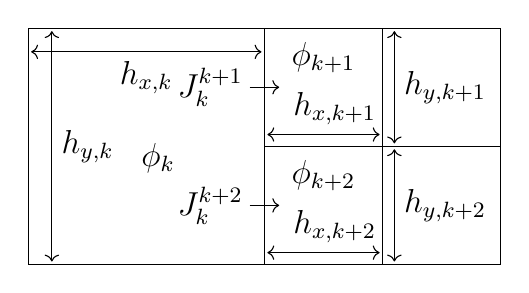
\begin{tikzpicture}[scale=0.75]
        
        %One nodes
        \draw[-] (0,0) -- (0,4) -- (4,4) -- (4,0) -- (0,0);
        \draw[-] (4,4) -- (8,4) -- (8,0) -- (4,0);
        \draw[-] (6,4) -- (6,0);
        \draw[-] (4,2) -- (8,2);
        
        \node at (2.2,1.8) {\large $\phi_{k}$};
        \node at (5.0,3.5) {\large $\phi_{k+1}$};
        \node at (5.0,1.5) {\large $\phi_{k+2}$};
        
        \draw[<->] (0.05,3.6) -- (3.95,3.6) node[pos=0.5,below] {\large $h_{x,k}$};
        
        \draw[<->] (0.4,0.05) -- (0.4,3.95) node[pos=0.5,right] {\large $h_{y,k}$};
        \draw[<->] (6.2,2.05) -- (6.2,3.95) node[pos=0.5,right] {\large $h_{y,k+1}$};
        \draw[<->] (6.2,0.05) -- (6.2,1.95) node[pos=0.5,right] {\large $h_{y,k+2}$};
    
        \draw[<->] (4.05,2.2) -- (5.95,2.2) node[pos=0.6,above] {\large $h_{x,k+1}$};
        \draw[<->] (4.05,0.2) -- (5.95,0.2) node[pos=0.6,above] {\large $h_{x,k+2}$};
    
        \draw[->] (3.75,3) -- (4.25,3) node[pos=0.1,left] {\large $J_{k}^{k+1}$};
        \draw[->] (3.75,1) -- (4.25,1) node[pos=0.1,left] {\large $J_{k}^{k+2}$};
        
    \end{tikzpicture}
    \caption{Semi-Structured Coarse Mesh}
    \label{fig:ssCM}
\end{figure}
%

It should be obvious that the semi-structured CMFD equations are a generalization of the structured coarse mesh case. The volume based quantities of \eqref{eq:homcoef} remain unchanged. However, the surface quantities from the discretized problem now have more general expressions that reduce correctly to \eqref{eq:dtil}, \eqref{eq:dhat}, and \eqref{eq:sCMFD} for the structured mesh case.

For the semi-structured grids, the equations for $\tilde D_g$, $\hat D_g$ and the balance equation are given as:

\begin{subequations} \label{eq:sscoef}
    \begin{equation}
        \tilde D_{g,k}^{k+n} = \frac{2\bar D_{g,k} \bar D_{g,k+n}}{
        h_{x,k+n} \bar D_{g,k} + h_{x,k} \bar D_{g,k+n} } ,
    \end{equation}
    \begin{equation}
        \hat D_{g,k}^{k+n} = \frac{ J_{g,k}^{k+n}
         + \tilde D_{g,k}^{k+n}\Big(\bar\phi_{g,k+n}-\bar\phi_{g,k}\Big)}
        {\Big(\bar\phi_{g,k}+\bar\phi_{g,k+n}\Big)} ,
    \end{equation}
    \begin{multline}
        \sum_{n=1}^{N} h_{z,k} h_{y,k+n}\left[\tilde D_{g,k}^{k+n} \left( \bar\phi_{g,k} - \bar\phi_{g,k+n} \right)  + \hat D_{g,k}^{k+n} \left( \bar\phi_{g,k} + \bar\phi_{g,k+n} \right) \right]
    \\ + V_{k}\bar\Sigma_{t,g,k}\bar\phi_{g,k} = V_{k} \bar Q_{g,k} .
    \end{multline}
\end{subequations}

\section{Implementation}
While the aspects of the theory for general unstructured applications was discussed, the present implementation in MPACT is limited to the semi-structured grids encountered in BWRs. This means we modify the conventional CMFD to explicitly treat cells with multiple neighbors per face, but not arbitrary polygons. Most of the work involved in modifying a code to go from PWR applications to BWR applications necessitates more sophisticated "book keeping" when performing ray tracing on the coarse mesh and calculating surface currents during the MOC sweep. Specifically, neighbor surface identification was handled in many places by the direction of the neighbor (north, east, west, south, top, and bottom). With a semi-structured mesh, this is no longer a unique identifier of a surface, so the coarse mesh surface index corresponding to the neighbor was used instead. The overall iteration scheme for the unstructured or semi-structured cases remains unchanged. Additionally, it should be noted that for 2D/1D formulations of the 3D transport equation, the calculation of the radial transverse leakage must also be modified.
%%%%%%%%%%%%%%%%%%%%%%%%%%%%%%%%%%%%%%%%%%%%%%%%%%%%%%%%%%%%%%%%%%%%%%%%%%%%%%%%
\section{Results and Analysis}
In this section we present some verification of the unstructured CMFD capability along with some results that demonstrate the method scales well up to a full BWR core.

%%%%%%%%%%%%%%%%%%%%%%%%%%%%%%%%%%%%%%%%%%%%%%%%%%%%%%%%%%%%%%%%%%%%%%%%%%%%%%%%
\subsection{Verification with Monte Carlo}
To verify the implementation of the method is correct we ran a 2x2 model of BWR lattices from Peach Bottom Unit 2 cycle 1 \cite{Larsen1978}. The model is shown in \figref{fig:pb2x2}. The Monte Carlo reference solution is provided by KENO \cite{SCALE2009} and two cases are simulated with MPACT using P2 scattering; one with the semi-structured CMFD acceleration employing the recently developed MSED solver \cite{Yee2017}, and one with just standard source iteration (SI). We compare the eigenvalue and run times for each case in \ref{tab:pb2x2}. The KENO case used 96 processors, while MPACT used 4 processors.

\begin{figure}[!ht]
    \centering
    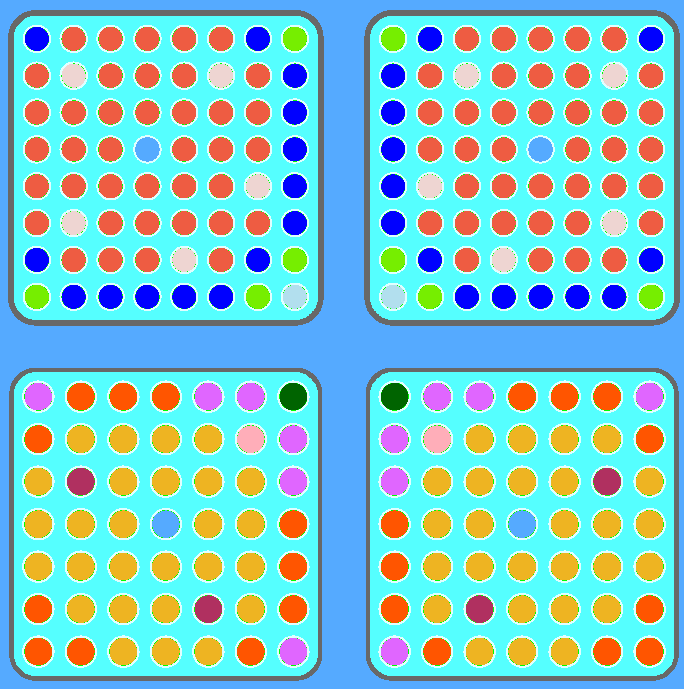
\includegraphics[width=0.2\textwidth]{pb-2x2-cropped.png}
    \caption{Peach Bottom 2x2 Mixed Lattice Configuration}
    \label{fig:pb2x2}
\end{figure}
\begin{table}[!htb]
    \centering
    \renewcommand{\arraystretch}{1.45}
    \caption{$k_{\text{eff}}$ and run times of Peach Bottom 2x2 Model}
    \label{tab:pb2x2}
    \begin{tabular}{@{}ccc@{}}\toprule
      Method        & $k_{\text{eff}}$ ($\Delta k$ in pcm)  & CPU-hours\\\midrule
      KENO CE       & 1.08922 ($\pm$2)  & 335.365\\
      MPACT SI      & 1.08655 (-267)    & 7.333\\
      MPACT CMFD    & 1.08655 (-267)    & 0.346\\\bottomrule
    \end{tabular}
    \vspace{-2mm}
\end{table}

From these results we see that MPACT produces consistent answers with and without CMFD and that the semi-structured CMFD is still an effective accelerator (21x speedup). For the max absolute and root-mean-square pin power errors both MPACT cases were 1.38\% and 0.49\%, respectively. The difference compared to KENO is consistent with previous results \cite{Kochunas2017} and reflects the current state of the cross section library for applications to BWRs.

%%%%%%%%%%%%%%%%%%%%%%%%%%%%%%%%%%%%%%%%%%%%%%%%%%%%%%%%%%%%%%%%%%%%%%%%%%%%%%%%
\subsection{Demonstration on a 2D BWR Core}
To demonstrate the effectiveness and robustness of the method, a 2D full core BWR model based on Peach Bottom, is simulated. The case was first run for cycle 1 under HFP conditions and 40\% void with all rods out and no feedback. The core is depleted to 10.0 GWD/MT, then the fuel is shuffled and an approximate beginning of cycle (BOC) condition for cycle 2 is simulated.

The cycle depletion was run with 22 state points on 222 processors on the Falcon cluster at INL. The total solve time was 3.4 hours. To both demonstrate and verify the shuffle, the end of cycle (EOC) 1 exposures and BOC 2 exposures after shuffle are shown in \figref{fig:pb_shuffle}. The BOC 2 case with the semi-structured CMFD converged in 17.16 minutes on 222 processors. By comparison for BOL conditions the Peach Bottom case takes 199 seconds, a 2D full core PWR, with a structured CMFD grid, on 222 processors takes 128 seconds.

\begin{figure}[!ht]
    \centering
    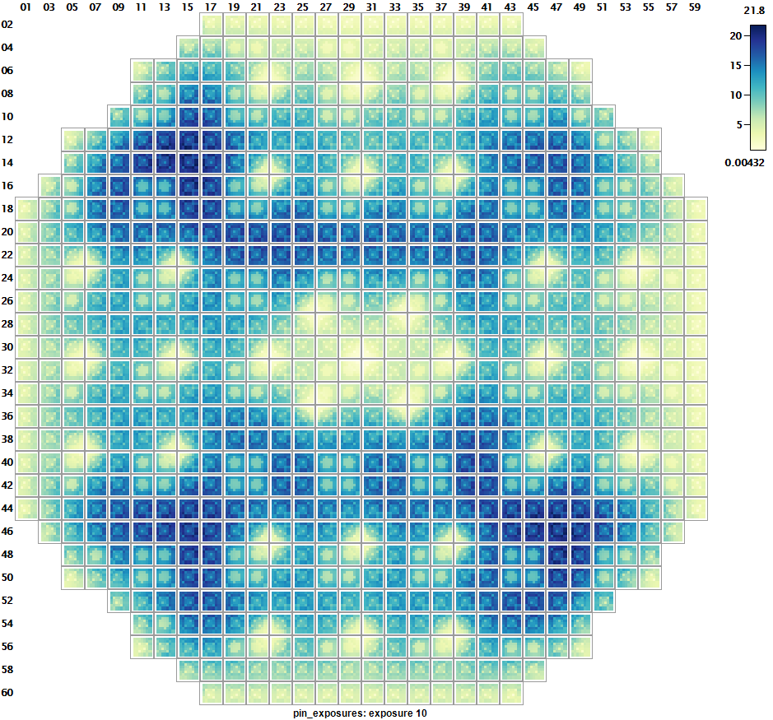
\includegraphics[width=0.22\textwidth]{pin_exposures_PB_Cycle1_2D_EOC.png}
    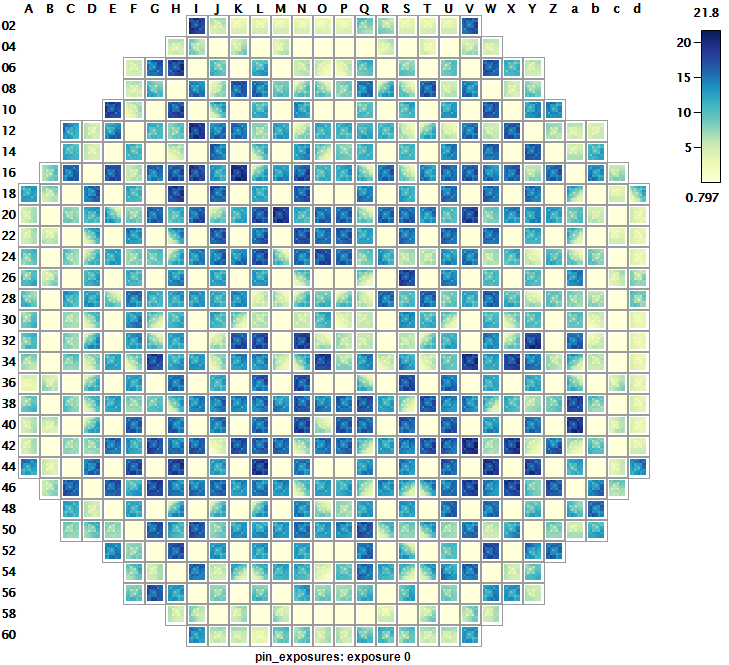
\includegraphics[width=0.22\textwidth]{pin_exposures_PB_Cycle2_2D_BOC.png}
    \caption{Peach Bottom Unit 2 Cycle 1 EOC (Left) and Cycle 2 BOC (Right)}
    \label{fig:pb_shuffle}
\end{figure}

%%%%%%%%%%%%%%%%%%%%%%%%%%%%%%%%%%%%%%%%%%%%%%%%%%%%%%%%%%%%%%%%%%%%%%%%%%%%%%%%
\section{Conclusions}
The aspects of structured and unstructured CMFD are presented and discussed. The necessary treatments for modeling BWRs with a pin-wise CMFD only requires treatment of a semi-structured grid. Purely unstructured CMFD methods have relied on approximate or inconsistent discretizations that may require "fix-ups" for improved robustness at the cost of efficiency. Some potential candidates for a rigorous unstructured CMFD capability are given, although the need for a rigorous unstructured CMFD capability is suspect.
The implementation of the semi-structured CMFD capability in MPACT is described and verified against Monte Carlo results from KENO. The capability is also demonstrated for a 2D full core BWR multi-cycle simulation. The semi-structured CMFD capability in MPACT is shown to be efficient and robust. Future work might focus on evaluating the benefits of a consistent CMFD discretization for various types of meshes.

%%%%%%%%%%%%%%%%%%%%%%%%%%%%%%%%%%%%%%%%%%%%%%%%%%%%%%%%%%%%%%%%%%%%%%%%%%%%%%%%
\section{Acknowledgments}
This research was supported by the Consortium for Advanced Simulation of Light Water Reactors (www.casl.gov), an Energy Innovation Hub (http://www.energy.gov/hubs) for Modeling and Simulation of Nuclear Reactors under U.S. Department of Energy Contract No. DE-AC05-00OR22725. This research also made use of the resources at the High Performance Computing Center at Idaho National Laboratory, that is also supported by the Office of Nuclear Energy of the U.S. Department of Energy and the Nuclear Science User Facilities under Contract No. DE-AC07-05ID14517.

%%%%%%%%%%%%%%%%%%%%%%%%%%%%%%%%%%%%%%%%%%%%%%%%%%%%%%%%%%%%%%%%%%%%%%%%%%%%%%%%
\bibliographystyle{ans}
\bibliography{bibliography}
\end{document}

